% 百科创作指导
% 小时百科|词条|目录|预备知识|目录树|参考文献

\subsection{内容创作}
\begin{itemize}
\item 请遵守 “小时百科符号与规范\upref{Conven}”.
\item 新志愿者建议先在群里(或者和管理员)讨论内容和构思再开始写.
\item 新建词条以前必须确认无重复内容, 若创作了相同内容且质量并不更好, 将会被删除.
\item 如果当前内容只是一个大纲或草稿, 需要标记为草稿词条(在 \verb|issues| 环境中插入 \verb|\issueDraft|).
\item 小时百科是一个侧重于自学的百科. 所以内容需要尽量对初学者友好, 例如足够的文字讲解, 图片, 例题等. 如果只是简单的堆砌公式定理, 需要标记词条为 “需要更多讲解” (在 \verb|issues| 环境中插入 \verb|issueAbstract|).
\item 在正文的任何地方可以用 \verb|\addTODO{}| 来插入需要补充的内容, 如果这么做, 同时需要将词条标记为 “存在未完成内容”(在 \verb|issues| 环境中插入 \verb|\issueTODO|).
\item 如果 TODO 的内容不希望被读者看到, 可以直接用注释, 但需要包含 “未完成” 三个字.
\item 可以在 \verb|issues| 环境中用 \verb|\issueOther{}| 添加自定义 issue.
\item 注意词条中除了可以用 “内部引用” 按钮(实心冒号图标)一键引用本文的公式图表等, 也可以用 “外部引用” 引用其他词条的内容.
\end{itemize}

\subsection{目录}
\begin{itemize}
\item 请在文件 \verb|main.tex| 中修改目录.
\item 由于词条繁多, 小时百科目录中的 “部分” 和 “章节” 只是给所有内容做一个话题分类, 而不是按照建议阅读顺序排列. 建议的阅读顺序由下面介绍的 “预备知识” 决定.
\end{itemize}

\subsection{预备知识}
\begin{figure}[ht]
\centering
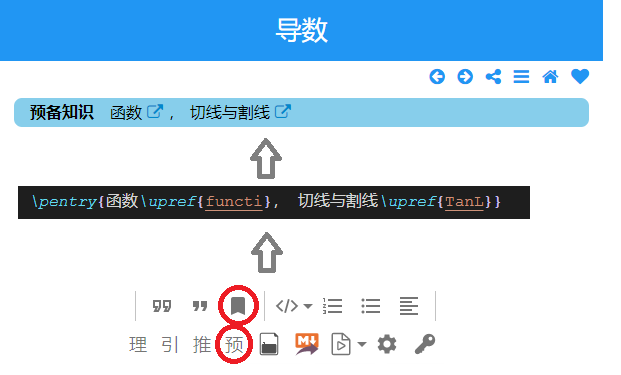
\includegraphics[width=13cm]{./figures/WrGuid_1.png}
\caption{使用菜单栏的按钮添加预备知识} \label{WrGuid_fig1}
\end{figure}

\begin{itemize}
\item 小时百科重视内容的自洽性, 所以几乎所有词条都需要指定其他一些词条作为预备知识(\autoref{WrGuid_fig1} ). 预备知识相当于 “必备知识”, 如果其中的内容不掌握, 读者阅读词条内容就会遇到较大的困难(例如从来没见过的术语,公式或定理).
\item 一般来说我们假设读者具有普通高中毕业生的数理水平. 任何超出该水平的内容都需要在 “预备知识” 中有所体现. 如果需要低于该水平的预备知识且存在相关词条, 也需要加入.
\item 注意百科词条目录并不按照建议阅读的顺序来排序而是按照话题排序, 且不鼓励读者按目录顺序阅读, 所以不能假设读者以已经读过当前词条前面的词条.
\item \href{http://wuli.wiki/tree/}{词条目录树}页面将自动按照 “预备知识” 生成. 读者可以把任意词条作为目标或起点生成该词条相关的知识树(\autoref{WrGuid_fig3} ).
\end{itemize}

\begin{figure}[ht]
\centering
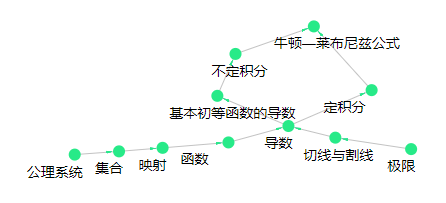
\includegraphics[width=12cm]{./figures/WrGuid_3.png}
\caption{由 “牛顿—莱布尼兹公式” 为目标生成的知识树} \label{WrGuid_fig3}
\end{figure}

\begin{itemize}
\item 注意 “预备知识” 是递归的,意味着你可以默认读者已经掌握 “预备知识” 词条中的 “预备知识”. 如果当前词条的预备知识里面已经列出了词条 A, 而词条 A 的预备知识中含有词条 B, 那么就无需把 B 再次列为当前词条的预备知识. 管理员会在后台定期检测到这些重复并协助删除这些多余的预备知识.
\item 即使一些术语在预备知识树中提到过, 也鼓励尽量添加链接以防遗忘.
\item 一些拓展或者选读性质的词条不需要作为预备知识, 例如 “详见……词条”.
\item 在添加预备知识时, 先浏览一下里面的内容, 确保它包含当前词条所需内容.
\item 如果百科中找不到预备知识所需的词条, 应该把当前词条标记为 “缺少预备知识” (\autoref{WrGuid_fig2}), 并用注释说明需要什么内容作为预备知识.
\end{itemize}

\begin{figure}[ht]
\centering
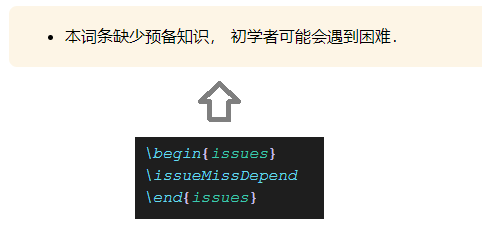
\includegraphics[width=13cm]{./figures/WrGuid_2.png}
\caption{将词条标记为 “缺少预备知识”} \label{WrGuid_fig2}
\end{figure}

\subsection{参考文献}
\begin{itemize}
\item 在 \verb|bibliography.tex| 的文献列表中添加你需要的参考文献, 然后在词条中用 \verb|\cite| 引用即可. 如果文献没有在正文中直接被引用, 那么可以在正文开始用 \verb|foornote| 添加, 如\footnote{本文参考 \cite{GriffE}, \cite{GriffQ} 以及 Wikipedia \href{https://www.wikipedia.org/}{相关页面}}.
\item 原则上每个词条都需要参考文献, 如果没有足够的文献, 需要标记为 “缺少参考文献”(在 \verb|issues| 环境中插入 \verb|\issueNeedCite|)
\item 一般来说比较方便的做法是直接引用 Wikipedia 相关页面(注意尽量选用质量更高的英文版), 读者可以参考由 Wikipedia 列出的更多参考文献.
\end{itemize}
